\documentclass[12pt,a4paper, spanish]{article}
% Sacar draft para que aparezcan las imagenes.
% Opciones: 12pt, 10pt, 11pt, landscape, twocolumn, fleqn, leqno...
% Opciones de clase: article, report, letter, beamer...

% Paquetes:
% =========
\usepackage[headheight=110pt, top = 2cm, bottom = 2cm, left=1cm, right=1cm]{geometry} %modifico márgenes
\usepackage[T1]{fontenc} % tildes
\usepackage[utf8]{inputenc} % Para poder escribir con tildes en el editor.
\usepackage[english]{babel} % Para cortar las palabras en silabas, creo.
\usepackage[ddmmyyyy]{datetime}
\usepackage{amsmath} % Soporte de mathmatics
\usepackage{amssymb} % fuentes de mathmatics
\usepackage{array} % Para tablas y eso
\usepackage{caption} % Configuracion de figuras y tablas
\usepackage[dvipsnames]{xcolor} % Para colorear el texto: black, blue, brown, cyan, darkgray, gray, green, lightgray, lime, magenta, olive, orange, pink, purple, red, teal, violet, white, yellow.
\usepackage{graphicx} % Necesario para poner imagenes
\usepackage{enumitem} % Cambiar labels y más flexibilidad para el enumerate
\usepackage{tikz} % para graficar
\usepackage{cancel}
\usepackage{titlesec} % para editar titulos y hacer secciones con formato a medida
\usepackage{ulem}
\usepackage{centernot} % tacha cosas
\usepackage{bbding} % símbolos de donde uso FiveStar
\usepackage{skull} % símbolos de donde uso Skull
% \usepackage{lipsum}
\usepackage{soul} % para tachar en mathmode -> \hbox{\sout{$x+1$}}

% para hacer los graficos tipo grafos
\usetikzlibrary{shapes,arrows.meta, chains, matrix, calc, trees, positioning, fit}
\usetikzlibrary{external,angles,quotes}

\setlength{\parindent}{0pt} % Para que no haya indentación en las nuevas líneas.

\begin{document}
% Definiciones y nuevos comandos:
% =============
\def\partes{\mathcal P}
\def\relacion{\,\mathcal{R}\,}
\def\norelacion{\,\cancel{\relacion}\,}
\def\universo{\mathcal U}
\def\reales{\mathbb R}
\def\naturales{\mathbb N}
\def\enteros{\mathbb Z}
\def\complejos{\mathbb C}
\def\i{\text{i}}
\def\vacio{\varnothing}
\def\union{\cup}
\def\inter{\cap}
\def\y{\land}
\def\o{\lor}
\def\neg{\sim}
\def\entonces{\Rightarrow}
\def\sisolosi{\iff}
\def\clase{\overline}


\def\existe{\,\exists\,}
\def\noexiste{\,\nexists\,}
\def\paratodo{\forall}
\def\distinto{\neq}
\def\en{\in}
\def\talque{\;|\;}

% =====
\def\qvq{\text{ quiero ver que }}

%funciones
\def\imagen{\text{Im}}
\def\dominio{$\text{Dom}$}
\def\comp{\circ}
\def\inv{^{-1}}
\def\infinito{\infty}

% Llaves, paréntesis, contenedores
\newcommand{\llave}[2]{ \left\{ \begin{array}{#1} #2 \end{array}\right. }
\newcommand{\llaves}[2]{ \left\{ \begin{array}{#1} #2 \end{array} \right\} }
\newcommand{\matriz}[2]{\left( \begin{array}{#1} #2 \end{array} \right)}
\newcommand{\deter}[2]{\left| \begin{array}{#1} #2 \end{array} \right|}
\newcommand{\lista}[2][(1)]{\begin{enumerate}[\bf #1]\setlength\itemsep{-0.6ex} #2 \end{enumerate}}
\newcommand{\listal}[2][-0.6ex]{\begin{enumerate}[\bf(a)]\setlength\itemsep{#1} #2 \end{enumerate}}

% naturales
\newcommand{\sumatoria}[2]{\sum\limits_{#1}^{#2}}
\newcommand{\productoria}[2]{\prod\limits_{#1}^{#2}}
\newcommand{\kmasuno}[1]{\underbrace{#1}_{k+1\text{-ésimo}}}
\newcommand{\HI}[1]{\underbrace{#1}_{\text{HI}}}

% enteros
\def\divide{\,|\,}
\def\congruente{\, \equiv \,}
\newcommand{\congruencia}[3]{#1 \equiv #2 \;(\text{mod}\;#3)}
\newcommand{\divset}[2]{\mathcal{D}(#1) = \set{#2}}



% =====
% Miscelanea
% =====
\newcommand{\estabien}{{\color{blue} Consultado, está bien. \checkmark}}
\newcommand{\hacer}{{\color{black!30!red}Hacer!}}
\newcommand{\Hacer}{{\color{black!30!red}\Large Hacer!}}

\def\llamadaI{\stackrel{\cyan{$*^1$}}}
\def\llamadaII{\stackrel{\cyan{$*^2$}}}
\def\llamadaIII{\stackrel{\cyan{$*^3$}}}

% separador
\def\separador{\noindent\rule{\linewidth}{0.4pt}\\}
\def\separadorCorto{\noindent\rule{0.5\linewidth}{0.4pt}\\}

% sección ejercicio con su respectivo formato y contador
\newcounter{ejercicio}[subsubsection] % contador que se resetea en cada sección
\renewcommand{\theejercicio}{\arabic{ejercicio}} % el contador es un número arabic
\newcommand{\ejercicio}{%
	\stepcounter{ejercicio}% incremento en uno
	\titleformat{\section}[runin]{\normalfont\bfseries}{\theejercicio}{1em}{}%
	\section*{\noindent\theejercicio. \noindent}%
}

% Colores
\newcommand{\red}[1]{ {\color{red} \text{#1}}}
\newcommand{\green}[1]{ {\color{olive} \text{#1}}}
\newcommand{\blue}[1]{ {\color{blue} \text{#1}}}
\newcommand{\cyan}[1]{ {\color{cyan} \text{#1}}}
\newcommand{\magenta}[1]{ {\color{magenta} \text{#1}}}

% Conjuntos entre llaves
\newcommand{\set}[1] { \left\{ #1 \right\} }
\newcommand{\parentesis}[1] { \left( #1 \right) }

% Stackrel text
\newcommand{\stacktext}[2]{ \stackrel{\text{#1}}{#2} }
\def\eq?{\stackrel{\text{?}}}

% Flecha con texto
\NewDocumentCommand{\flecha}{m o}{%
	\IfNoValueTF{#2}{%
		\xrightarrow[]{\text{#1}}
	}{
		\xrightarrow[\text{#2}]{\text{#1}}
	}
}
 % idem con las definiciones

\pagestyle{empty} % Para que no muestre el número en pie de página

% Info para armar título.
\title{Práctica 6 de álgebra 1} % título
\author{D. Garraz} % autor
\date{last update: \today} % Cambiar de ser necesario

\maketitle  % para que aprezca el título en el documento

\newpage
\section{Definiciones y fórmulas útiles}
\textit{\underline{Raíces de un número complejo: }}
\begin{itemize}
	\item Sean $z, w \en \complejos -\set{0}$, $z = re^{\theta i}$ y $w = se^{\varphi i }$ con $r,\, s \en \reales_{>0}$
	      y $\theta,\, \varphi \en \reales$.\\ Entonces $z = w \sisolosi
		      \llave{l}{
			      r = s\\
			      \theta = \varphi + 2 k\pi,\ \text{para algún } k \en \enteros
		      }$
	\item raíces $n$-esimas: $w^n = z
		      \to
		      \llave{l}{
		      s^n = r \\
		      \varphi \cdot n = \theta + 2 k \pi \quad\to \text{para algún $k\en \enteros$}\\
		      \text{$n$ raíces distintas} \to w_k=se^{\varphi_k i}, \text{ donde } s = \sqrt{r} \text{ y }
		      \varphi_k = \frac{\theta}{n} + \frac{2k\pi}{n} = \frac{\theta + 2k\pi}{n}


		      }$
\end{itemize}
\begin{itemize}
	\item $G_n = \set{w \en \complejos / w^n = 1} = \set{e^{\frac{2k \pi}{n} i}\ :\ 0\leq k \leq n-1}$

	\item $(G_n, \cdot)$ es un grupo abeliano, o conmutativo.
	      \begin{itemize}
		      \item $\paratodo w, z \en G_n, w z = z  w \text{ y } z m \en G_n$.

		      \item $1 \en G_n,\ w \cdot 1 = 1 \cdot w = w \qquad \paratodo w \en G_n$.

		      \item $w \en G_n \entonces \existe w^{-1} \en G_n,\ w \cdot w^{-1} = w^{-1}\cdot w = 1$
		            \begin{itemize}
			            \item $\conj w \en G_n,\ w \cdot \conj w = |w|^2 = 1 \entonces \conj w = w^{-1}$
		            \end{itemize}
	      \end{itemize}
	\item \textit{Propiedades: $w \en G_n$}
	      \begin{itemize}
		      \item $m \en \enteros$ y $n \divideA m \entonces w^m = 1$.

		      \item $\congruencia{m}{m'}{n} \entonces w^m = w^{m'}\quad (w^m = w^{r_n(m)})$

		      \item $n \divideA m \sisolosi G_n \subseteq G_m$

		      \item $G_n \inter G_m = G_{(n:m)}$

		      \item Si $(G, \cdot)$ es un grupo y $\#G = n$ decimos que $G$ siempre es cíclico si
		            $\existe w\en G / G = \set{1,w, w^2,\dots, w^{n-1}}$\\
		            \begin{itemize}
			            \item \textit{Observación: } $G_n$ es un grupo cíclico, ej, $w_1 = e^\frac{2\pi i}{n} \to (w_1)^k = w_k$\\
			                  $\to$ las potencias de $w_1$ generan todo $G_n = \set{1, w_1, w_1^2,\dots,w_1^{n-1}}$
		            \end{itemize}

		      \item $w$ es raíz $n-$ésima primitiva de 1 si:
		            $G_n = \set{1,w,w^2,\dots,w^{n-1}} =
			            \set{w^k\ :\ 0\leq k \leq n-1}$\\
		            Ejemplo: $i, -i$ son primitivas de $G_4 = \set{1,i,-1,-i} = \set{i^k\ :\ 0 \leq k \leq 3}$, pero 1 y -1 no son raíces primitivas de $G_4$.
	      \end{itemize}
	\item \textit{Definición: }
	      Sea $w$ una raíz primitiva de orden $n$ (el orden de
	      $w \en G_n,\, \text{ord}(w) = \text{min}\set{k \en \naturales / w^k = 1}$)
	      \begin{itemize}
		      \item $w^m = 1 \sisolosi n \divideA m$
		      \item \textit{Observación: } Si $w \en G_n \entonces \ord(w) \divideA n$
	      \end{itemize}
	\item La suma de las raíces $n$-ésimas de 1 da:
	      $\sumatoria{k=0}{n-1}w_1^k = \frac{w_1^n -1}{w_1 -1} = 0$ pues $w_1 \distinto 1$
	\item El producto de las raíces $n$-ésimas de 1 da:
	      $\productoria{k=0}{n-1} w_1^k = w_1^{0+1+\dots + n-1} =
		      w_1^{\frac{n(n-1)}{2}} =
		      \llave{rl}{
			      1 & \text{si $n$ es impar}\\
			      -1 & \text{si $n$ es par}
		      }$
	\item Sea $w \en G_n$ primitiva. Entonces
	      \begin{itemize}
		      \item $w^k \text{ es primitiva } \sisolosi k \cop n $
		      \item $w_k = e^{\frac{2k\pi}{n}i}$ es primitiva $\sisolosi k \cop n$
		      \item En particular para $n = p$ primo: $w_k$ es primitiva para $1\leq k < p$ o sea si
		            $w \en G_p$ y $w \distinto 1$, entonces $w$ es primitiva
	      \end{itemize}
	\item $w$ es raíz primitiva de $G_n$ y $k \divideA n \entonces w^k$ es primitiva de $G_\frac{n}{k}$
\end{itemize}

\subsubsection*{Ejercicios dados en clase:}
\ejercicio
Para $w \en G_6$, calcular $S = w^{71} + w^{-14} + 5\conj w^4 + w^{39} - 4w^{-22} + w^{2023}$

\separadorCorto
\textit{Si $w = 1$: }\\
$S = 5$\\

\textit{Si $w = -1$: }\\
$S = -1 + 1 + 5 - 1 -4 -1 = -1$\\

\textit{Si $w \distinto \pm 1$: }\\
$S = w^{71} + w^{-14} + 5\conj w^4 + w^{39} - 4w^{-22} + w^{2023} =
	w^5 + w^4 + 5 w^2 + w^3 - 4w^2 + w^1 =\\
	w^1 + w^2 + w^3 + w^4 + w^5 = \magenta{$-1$} + \ub{\magenta{$1$} + w^1 + w^2 + w^3 + w^4 + w^5}{=0} = -1$


\ejercicio
Sea $w \en G_{14}.$ Hallar todos los posibles valores de $w^7 + \sumatoria{j=7}{140}w^{2j}$

\separadorCorto
\text{Si $w = 1$}:\\
$w^7 + \sumatoria{j=7}{140} w^{2j} = 1 + 134 = 135$\\

\text{Si $w = -1$}:\\
$w^7 + \sumatoria{j=7}{140} w^{2j} = -1 + 134 = 133$\\

\text{Si $w \distinto \pm1$}:\\
$w^7 + \sumatoria{j=7}{140} w^{2j} =
	w^7 + \sumatoria{j=0}{140} (w^{2})^j - \sumatoria{j=0}{6} (w^2)^j =
	w^7 + \frac{(w^2)^{141} - 1}{w^2 - 1} - (1 + (w^2)^1 + (w^2)^2 + (w^2)^3 + (w^2)^4 + (w^2)^5 + (w^2)^6)
	\\
	\llave{l}{
		\text{Si } w = e^{i\frac{2k\pi}{14}} \text{ con } k\en [0,2,4,6,8,10,12]
		\entonces 1 + 1 - \ub{(1 + (w^2)^1 + (w^2)^2 + (w^2)^3 + (w^2)^4 + (w^2)^5 + (w^2)^6)}{ = 0} = 0\\
	}
$

\newpage

%=========================
% Ejercicios guia
%=========================

\section*{Ejercicios de la guía:}
\setcounter{ejercicio}{0} % Reset the custom counter

%1
\ejercicio

\setcounter{ejercicio}{6}

%7
\ejercicio
Hallar todos los $n \en \naturales$ tales que
\begin{enumerate}[label=\roman*)]
	\begin{minipage}{0.7\textwidth}
		\item $(\sqrt3 -i)^n = 2^{n-1}(-1 + \sqrt3 i)$ \\
		\separadorCorto
		$(\sqrt3 -i)^n = 2^n e^{i\frac{11}{12}\pi n} = 2^{n+1}\cdot 2e^{i \frac{2}{3} \pi}\\
			\to
			\llave{l}{
				2^n = 2^n\\
				\frac{11}{12}\pi n = \frac{2}{3}\pi + 2k \pi \to 11n = 8+8k \flecha{8(k+1)} \boxed{\congruencia{n}{0}{8}}
			}$
	\end{minipage}

	\item $(-\sqrt3 + i)^n \cdot \parentesis{\frac{1}{2} + \frac{\sqrt3}{2}i}$ es un número real negativo.\\
	      \separadorCorto
	      Un número real negativo tendrá un arg$(z) = \pi$\\
	      $\ub{(-\sqrt3 + i)^n}{2^ne^{i\frac{5}{6}\pi n}} \cdot \ub{\parentesis{\frac{1}{2} + \frac{\sqrt3}{2}i}}{e^{\frac{\pi}{3}i}} =
		      2^ne^{i(\frac{5}{6}n + \frac{1}{3}) \pi} \to \theta = (\frac{5}{6}n + \frac{1}{3}) \pi $\\
	      $\flecha{$\theta = \pi + 2k\pi$}
		      \cancel\pi \frac{5}{6}n + \frac{\cancel\pi}{3} = \cancel\pi + 2k\cancel\pi
		      \flecha{acomodo}[congruencia]
		      \congruencia{5n}{4}{12}
		      \flecha{multiplico}[por 5]
		      \boxed{\congruencia{n}{8}{12}} $

	\item $\text{arg}((-1+i)^{2n}) = \frac{\pi}{2}$ y $\text{arg}((1-\sqrt3 i)^{n-1}) = \frac{2}{3}\pi$

	      \separadorCorto
\end{enumerate}
\setcounter{ejercicio}{8}

%9
\ejercicio
Hallar todos los $z \en \complejos$ tales que $3z^5 + 2|z|^5 + 32 = 0$

\separadorCorto
$3 z^5 + 2|z|^5 +32 = 0
	\to
	\ub{3z^5}{\en \complejos} = \ub{-2|z|^5- 32}{\en \reales}
	\sisolosi
	\llaves{l}{
		\re(3z^5) =  -2|z|^5 - 32\\
		\im(3z^5) =  0
	} \Tilde$\\

\textit{De la ecuación de la parte imaginaria: }\\
$\llave{l}{
		\im(3z^5) = 3 \cdot \frac{z^5 - \conj z^5}{2} = 0
		\sisolosi
		z^5 = \conj z^5
		\sisolosi
		|z|^5 e^{5 \theta i} = |z|^5 e^{-5 \theta i}
		\sisolosi
		\llave{l}{
			5 \theta = -5 \theta + \magenta{$2k\pi$}\\
			\to \boxed{\theta_k = \frac{1}{5}k\pi} \text{ con } k \en [0,4]
		}
	}$\\

\textit{De la ecuación de la parte real: }\\
$\llave{l}{
		\re(3z^5) = 3 \cdot \frac{z^5 + \conj z^5}{2} =
		3 \cdot \frac{|z|^5 e^{5\theta i} + |z|^5 e^{-5\theta i}}{2} =
		3|z|^5 \cos(5\theta) =  -2|z|^5 - 32 \sii\\
		\sii
		|z|^5(3\cos(5\theta) + 2) = -2^5
		\flecha{evaluando}[en $\theta_k$]
		|z|^5(3\cos(k\pi) + 2) = -2^5
		\llave{cl}{
			\flecha{$k$}[par]     & 0 < |z|^5(3 + 2) \distinto -2^5 \quad \skull\\
			\flecha{$k$}[impar]   & |z|^5(-3 + 2) = -2^5 \sii |z| = 2
		}
	}\\
	\to$
\boxed{z_k = 2 e^{\theta_k i}} con $\theta_k = \frac{1}{5}k\pi \text{ con } k \en [0,4]$


%10
\ejercicio
Hallar todos los $n \en \naturales$ para los cuales la ecuación $z^n + i\conj z^2 = 0$,
tenga exactamente 6 soluciones y resolver en ese caso.

\separadorCorto
$\flecha{acomodo la }[ecuación]
	z^n = -i\conj z^2
	\flecha{$r = |z|$, expreso todo}[en notación exponencial]
	\llaves{l}{
		z^n = r^n e^{n  \theta i} \\
		\conj z^2 = r^2 e^{-2\theta i} \\
		-i = e^{\frac{3}{2}\pi}
	}\checkmark\\
	\flecha{reescribo ecuación con}[notación exponencial]
	r^n e^{n \theta i} = r^2 e^{(\frac{3}{2}\pi - 2\theta)i}
	\sisolosi
	\llaves{l}{
		n \theta =\frac{3}{2}\pi - 2\theta  + \magenta{$2k\pi$}\quad (k \en \enteros)\\
		r^n = r^2 \to r^2 (r^{n-2} - 1) = 0
	}$\\

\textit{La ecuación de $r$: }\\
$r = 0$ aporta una solución trivial para cualquier $n \en \naturales$.\\
$r = 1$ es un comodín que me deja usar cualquier $n$ para jugar con la ecuación de $\theta$.\\
$n = 2$ es un valor que daría una solución para cada $r \en \reales_{\geq 0}$. \underline{No sirve} porque necesito solo 6 soluciones.\\

\textit{La ecuación de $\theta$: }\\
$\flecha{$r = 1$}[$n$ libre] (n + 2)\theta = (\frac{3}{2} + 2k) \pi
	\flecha{$n+2 \distinto 0$}[$\paratodo n \en \naturales$]
	\theta = \frac{1}{n+2}(\frac{3}{2} + 2k) \pi
	\flecha{$n = 3$\red{ Cómo justificar esto elegantemente?}}[5 porciones de $2k\pi$]
	\theta = \frac{3 + 4k}{10} \pi
$\\
\textit{Las 6 soluciones para $n = 3$: }\\
$z^n + i\conj z^2 = 0 \sisolosi
	\llave{l}{
		n = 3\\
		z = 0,\, \text{ cuando } r = 0\\
		\text{ o }\\
		z_k = e^{\theta_k i} \text{ con } \theta_k = \frac{3 + 4k}{10} \pi ,\, k\en [0,4]
	}$


%11
\ejercicio
\textit{Voy a estar usando las siguientes propiedades en $G_n$: }\\
Si $w \en G_n \entonces
	\llave{l}{
		w^n = 1 \entonces w^k = w^{r_n(k)}\\
		\conj w^k = w^{r_n(-k)} \\
		\sumatoria{k=0}{n-1}w^k = 0\\
		m \divideA n \entonces G_m \subseteq G_n\\
		\text{Si } w \en G_p \text{ con $p$ primo} \entonces w \text{es primitiva}
		w^k \text{es primitiva} \sisolosi k \cop n
	}$\\
\begin{enumerate}[label=\roman*)]
	\item Calcular $w + \conj w + (w + w^2)^2 - w^{38}(1 - w^2)$ para cada $w \en G_7$.

	      \separadorCorto
	      \textit{Si} $w = 1$: \\
	      $w + \conj w + (w + w^2)^2 - w^{38}(1 - w^2) = 6$\\

	      \textit{Si} $w \distinto 1$: \\
	      $w + \ub{\conj w}{w^6} + (w + w^2)^2 - w^{38}(1 - w^2) =
		      w + w^6 + w^2 + 2w^3 + w^4 - \ub{(w^7)^5}{=1} w^3(1 - w^2) =\\
		      =  \magenta{$-1$} + \ub{\magenta{1} + w + w^2 + w^3 + w^4 + w^5 + w^6}{=0} = -1 \Tilde$

	\item Calcular $w^{73} + \conj w \cdot w^9 + 8$ para cada $w\en G_3$.

	      \separadorCorto
	      \textit{Si} $w = 1$: \\
	      $w^{73} + \conj w \cdot w^9 + 8 = 10 $\\

	      \textit{Si} $w \distinto 1$: \\
	      $\ub{w^{73}}{w} + \ub{\conj w \cdot w^9 }{w^2 \cdot 1}+ 8 =
		      \magenta{$-1$} + \ub{\magenta{1} + w + w^2}{= 0} + 8 = 7 $

	\item Calcular $1 + w^2 + w^{-2} + w^4 + w^{-4}$ para cada $w\en G_{10}$.

	      \separadorCorto
	      \red{Me falta harto golpe de horno para entender lo que pasa acá}\\
	      \red{¿Cómo tengo que interpretar la info de $G_5 \subseteq G_{10}$? está proveyendo}\\

	      \begin{minipage}{0.65\textwidth}
		      \textit{Si} $w = \pm1$: \\
		      $1 + w^2 + w^{-2} + w^4 + w^{-4} = 5$\\

		      \textit{Si} $w \distinto \pm1$: \\
		      $1 + w^2 + w^{-2} + w^4 + w^{-4} = 1 + w^2 + w^8 + w^4 + w^6\\
			      \llave{l}{
				      \flecha{\red{¿justificar?}}[\magenta{$G_5$}]
				      1 + w^2 + w^3 + w^4 + w^5 = 0\\
				      \flecha{\red{¿justificar?}}[\cyan{$G_5$}]
				      1 + \magenta{$1$} + \ub{\magenta{$-1$} + w^2 + w^3 + w^4 + w^5}{=0} = 2
			      }$
	      \end{minipage}
	      \begin{minipage}{0.4\textwidth}
		      $G_5 \subseteq G_{10}$\\
		      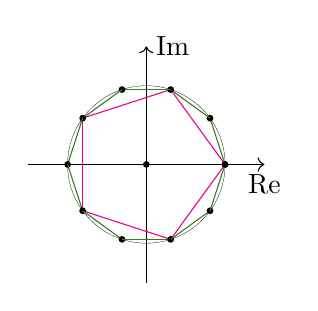
\begin{tikzpicture}[baseline=0]
			      \draw[->] (-1.5,0) -- (1.5,0) node[below] {Re};
			      \draw[->] (0,-1.5) -- (0,1.5) node[right] {Im};
			      \draw[ultra thin] (0,0) circle (1);
			      \filldraw[thin] (0,0) circle (1pt); % Added the origin
			      \foreach \x in {0,...,10} {
					      \filldraw (\x*360/10:1) circle (1pt);
					      \ifnum\x<10
						      \draw[OliveGreen] (\x*360/10:1) -- ({(\x+1)*360/10}:1);
					      \fi
					      \ifnum\x<5
						      \draw[magenta] (\x*360/5:1) -- ({(\x+1)*360/5}:1);
					      \fi
				      }
		      \end{tikzpicture}

		      $"G_5" \subseteq G_{10}$\\
		      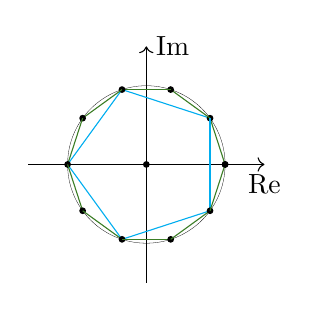
\begin{tikzpicture}[baseline=0]
			      \draw[->] (-1.5,0) -- (1.5,0) node[below] {Re};
			      \draw[->] (0,-1.5) -- (0,1.5) node[right] {Im};
			      \draw[ultra thin] (0,0) circle (1);
			      \filldraw[thin] (0,0) circle (1pt); % Added the origin
			      \foreach \x in {0,...,10} {
					      \filldraw (\x*360/10:1) circle (1pt);
					      \ifnum\x<10
						      \draw[OliveGreen] (\x*360/10:1) -- ({(\x+1)*360/10}:1);
					      \fi
					      \ifnum\x<5
						      \draw[cyan] ({\x*360/5+360/10}:1) -- ({(\x+1)*360/5+360/10}:1);
					      \fi
				      }
		      \end{tikzpicture}
		      \red{No tiene al 1? No es $G_5$}
		      \red{Solo vale el primer gráfico?}
		      \red{Condiciona los $w$ del ejercicio?}
	      \end{minipage}

	\item Calcular $w^{14} + w^{-8} + \conj w^4 + \conj{w^{-3}}$ para cada $w \en G_5$

	      \separadorCorto
	      \textit{Si} $w = 1$: \\
	      $w^{14} + w^{-8} + \conj w^4 + \conj{w^{-3}} = 4$

	      \textit{Si} $w \distinto 1$: \\
	      $w^{14} + w^{-8} + \conj w^4 + \conj{w^{-3}} =
		      w^4 + w^2 + w + w^3 =
		      \magenta{$-1$} + \ub{\magenta{1} + w + w^2 + w^3 + w^4}{= 0} = -1 $


\end{enumerate}
\newpage
%12
\ejercicio
\begin{enumerate}[label=\roman*)]
	\item Sea $w \en G_{36}$, $w^4 \distinto 1.$ Calcular $\sumatoria{k=7}{60}w^{4k}$

	      \separadorCorto
	      Sé que si $w \en G_{36} \entonces
		      \llave{l}{
			      w^{36} = 1 \\
			      \sumatoria{k=0}{35} w^k = 0
		      }$\\
	      Como $w^4 \distinto 1$ sé que $w \distinto \pm1$. Si no tendría que considerar casos particulares para la suma.\\

	      Si
	      $\sumatoria{k=7}{60}w^{4k} =
              \ub{\sumatoria{k=7}{60}w^{4k} + \magenta{$\sumatoria{k=0}{6}w^{4k}$}}{\sumatoria{k=0}{60}w^{4k}}
              - \magenta{$\sumatoria{k=0}{6}w^{4k}$} =
		      \sumatoria{k=0}{60}w^{4k} - \sumatoria{k=0}{6}w^{4k} =
		      \frac{(w^4)^{61} - 1}{w^4 - 1} - \frac{(w^4)^7 - 1}{w^4 - 1} =
		      \frac{(w^4)^{61} - (w^4)^7 }{w^4 - 1}\\
		      \flecha{$61 = 9\cdot6 + 7 $}[$w^36 = 1$]
              \frac{((\ob{ \scriptstyle w^{36}}{=1})^6  \cdot (w^4)^7 - (w^4)^7 }{w^4 - 1}
		      \to$
              \boxed{\sumatoria{k=7}{60}w^{4k} =0}

	\item Sea $w \en G_{11}$, $w \distinto 1.$ Calcular $\re\parentesis{\sumatoria{k=0}{60}w^k}$.

	      \separadorCorto
	      Sé que si $w \en G_{11} \entonces
		      \llave{l}{
			      w^{11} = 1 \\
			      \sumatoria{k=0}{10} w^k = 0\\
			      11 \text{ es impar} \entonces -1 \not\en G_{11}
		      }$\\
	      Como $w \distinto 1$ no calculo caso particular para la suma.
	      Me piden la parte real $ \flecha{uso} \re(z) = \frac{z + \conj z}{2}$.\\

	      Probé hacer la suma de Gauss como en el anterior, pero no llegué a nada, abro sumatoria y uso que $61 = 5 \cdot 11 +6$, porque hay 61 sumandos.\\

	      $\sumatoria{k=0}{60}w^k =
		      w^0 + \dots + w^{60} =
              5 \cdot \ub{\ob{(w^0 + w^1 + \dots + w^9 + w^{10})}{=0}}{\text{\tiny agrupé usando: }w \en G^{11} \entonces w^k = w^{r_{11}(k)}} +
		      w^{55} + w^{56} + w^{57} + w^{58} + w^{59} + w^{60}=\\
		      = w^0 + w^1 + w^2 + w^3 + w^4 + w^5 \llamada1
	      $\\

	      También voy a usar que si $w \en G_{11} \entonces \conj w^k = w^{r_{11}(-k)}$\\
	      $\re\parentesis{\sumatoria{k=0}{60}w^k +\sumatoria{k=0}{60}\conj w^k } \stackrel{\llamada1}=
		      w^0 + w^1 + w^2 + w^3 + w^4 + w^5 + \conj w^0 + \conj w^1 + \conj w^2 + \conj w^3 + \conj w^4 + \conj w^5 =\\
		      = w^0 + \ub{w^1 + w^2 + w^3 + w^4 + w^5 + w^0 + w^{10} + w^9 + w^8 + w^7 + w^6}{\sumatoria{k=0}{10} w^k} =
		      \ub{w^0}{1} + \ub{\sumatoria{k=0}{10} w^k}{= 0} = 1
	      $

\end{enumerate}
\end{document}
